%
	\chapter*{Motivation}\addchaptertocentry{Motivation}
%
        \begin{figure}[!b]
            \centering
            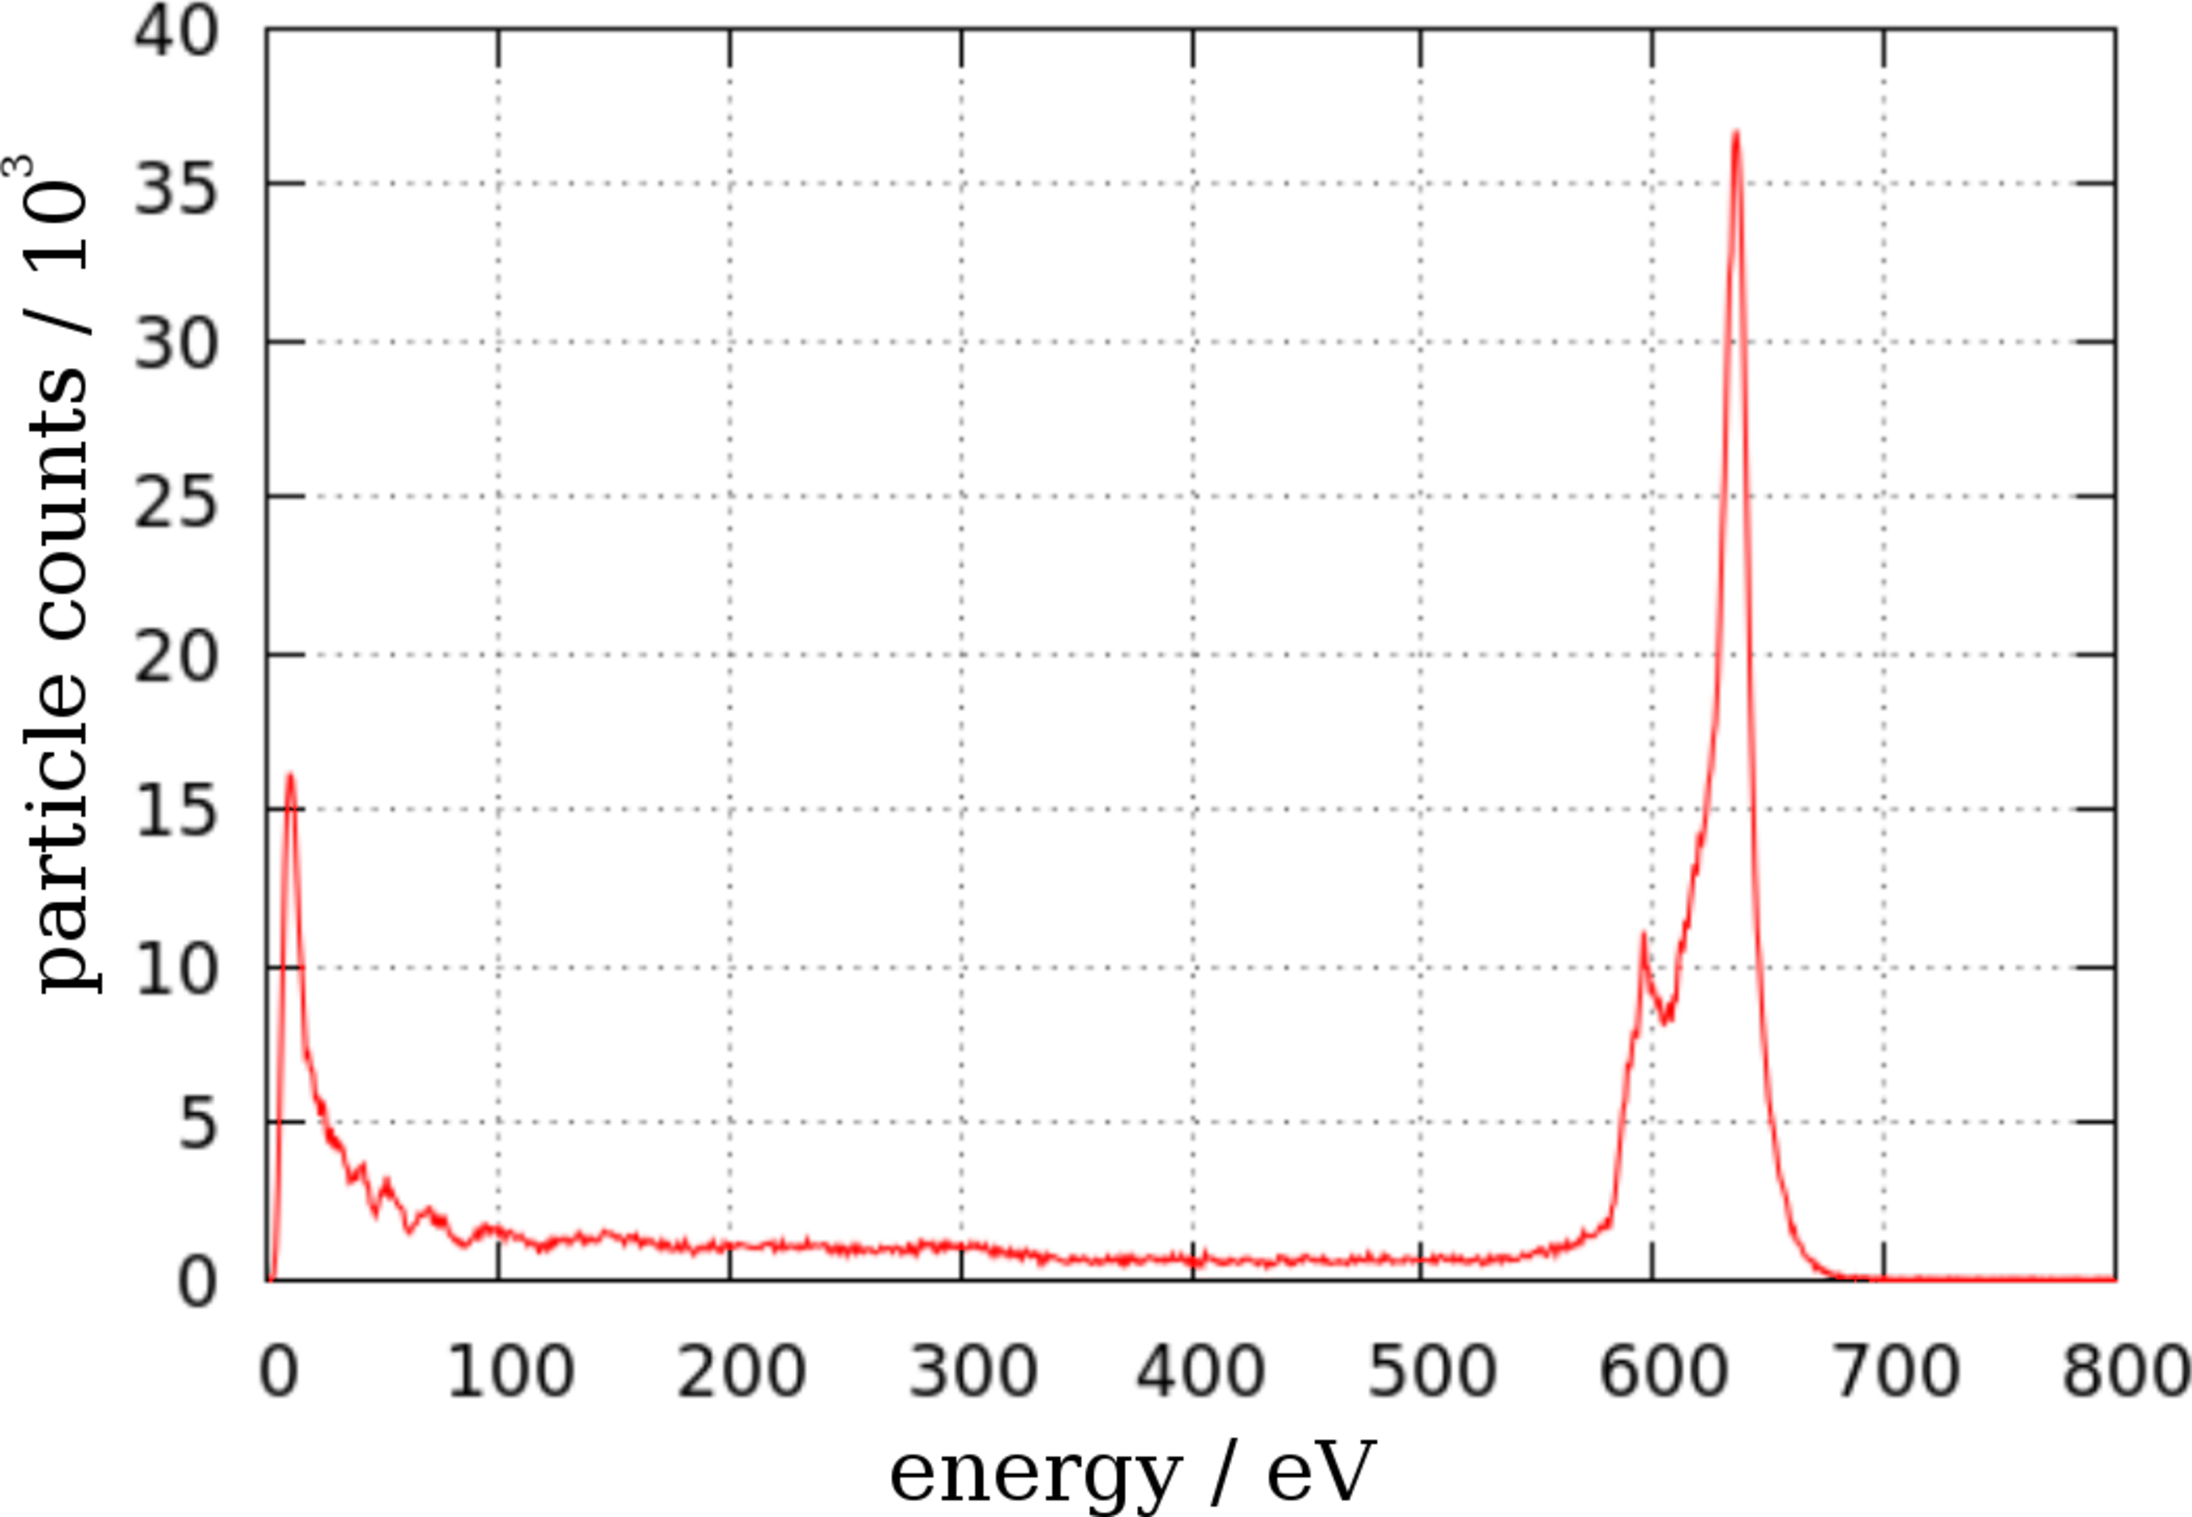
\includegraphics[width=.8\textwidth]{figures/scheuer_anionedf.pdf}
            \caption[Experimentally measured anion EDF at the anode]{%
                Experimentally measured anion energy distribution function impinging %
                on the grounded electrode. Magnesium oxide was used as cathode material, %
                which was powered with $\SI{50}{\watt}$~\cite{Scheuer15}.}
            \label{fig:anionedf_scheuer}
        \end{figure}
%
        Reactive plasmas are a common tool in many industrial and scientific applications, such as semiconductor and computer chip production. Of high importance for the surface treatment are etching and sputtering processes~\cite{Cvelbar05,Zeuner98}. Especially in electronegative discharges sputter and deposition rates are increased. They depend crucially on the distribution function of impinging ions. Therefore, a detailed understanding of these distribution functions is needed to optimise the processes. Capacitively coupled discharges with radio-frequency modulated voltages (ccrf) have high-energy ions impinging on the electrodes. Their advantage is the absence of a net current onto the target, which preserves the structure of the product.\\
        Laboratory experiments with ccrf oxygen discharges at low pressures and temperatures show a high-energy peak in the energy distribution function (EDF) of negative ions impinging on the anode. The position of this peak depends on the electrode material~\cite{Scheuer15}. Experimentally measured anion EDF is shown in~\autoref{fig:anionedf_scheuer}. A possible explanation is proposed by Stoffels and Kawano et al.~\cite{Stoffels01,Kawano83}: negative ions are produced by ionisation close to or at the surface of the electrode. The drawback of this theory is the lack of experimental or theoretical ionisation probabilities for anions at metal surfaces. Until now an explanation for this characteristic feature of the EDF of negative ions at the anode is missing.\\        
        In my thesis I will try to study this system and to improve the understanding of the underlying physics of the high-energy peak in the EDF of negative ions at a grounded electrode. Since the EDF is non-Maxwellian, a kinetic model is needed. Therefore, a Particle-in-Cell (PIC) code with Monte-Carlo-Collisions (MCC) is used to model the asymmetric ccrf discharges of low-temperature oxygen plasmas. In particular, an surface ionisation module for negative ions is introduced in the simulation and its effect on the EDF is studied.\\
        In this thesis I will try to answer the following questions:
      
        \begingroup\par
            \centering
            \bigskip\fbox{
                \parbox[c]{0.8\textwidth}{
                    \begin{enumerate}
                        \item What determines the physics of ccrf low pressure oxygen plasmas?
                        \item What is the influence of surface processes on the %
                                distribution function of negative ions?
                    \end{enumerate}
                }
            }
            \bigskip\par
        \endgroup
        
        Numerical investigations of electronegative plasmas have been done, e.g.\@ by~\cite{Matyash07oxIII,Bronold07b,Matthias15} using an one-dimensional PIC model. It has proven to be a great tool for fundamental studies of reactive radio frequency plasmas. Although this is a good approach for the investigation of axial distribution functions of plasma species close to the axis, the 1D simulations lacks effects of radial transport, asymmetry and plasma-wall interaction. For these topics, a 2D radial-axial model is needed, which is validated by comparison with the existing 1D code. In the 2D model, additional effects, such as voltage offset \emph{self bias} in ccrf discharges and asymmetry effects are taken into account.%
%        
        \par\bigskip
        To be able to answer the basic scientific question formulated before, I will firstly introduce the basic physics of plasmas in front of walls, the so-called plasma sheath. This will be extended to ccrf conditions, where the plasma reacts dynamically to the RF heating. The need for kinetic models to resolve the full distribution functions of all plasma species is satisfied by the PIC-MCC simulation method, which will be summarised shortly. As a part of the computational model, the relevant collision processes for such ccrf oxygen plasmas are discussed.\\
        In the second part of the thesis I will simulate the axial centre of the discharge without asymmetry effects using the one-dimensional model. These results are also used for a validation of the 2D radial-axial model.  After its successful validation the 2D model is used to simulate the experimental conditions of the plasma discharge from~\cite{Scheuer15}. In the PIC simulations, special emphasis lies on the investigation of surface and asymmetry effects and their impacts. Finally, the work is summarised.